\documentclass[twoside]{book}

% Packages required by doxygen
\usepackage{fixltx2e}
\usepackage{calc}
\usepackage{doxygen}
\usepackage[export]{adjustbox} % also loads graphicx
\usepackage{graphicx}
\usepackage[utf8]{inputenc}
\usepackage{makeidx}
\usepackage{multicol}
\usepackage{multirow}
\PassOptionsToPackage{warn}{textcomp}
\usepackage{textcomp}
\usepackage[nointegrals]{wasysym}
\usepackage[table]{xcolor}

% Font selection
\usepackage[T1]{fontenc}
\usepackage[scaled=.90]{helvet}
\usepackage{courier}
\usepackage{amssymb}
\usepackage{sectsty}
\renewcommand{\familydefault}{\sfdefault}
\allsectionsfont{%
  \fontseries{bc}\selectfont%
  \color{darkgray}%
}
\renewcommand{\DoxyLabelFont}{%
  \fontseries{bc}\selectfont%
  \color{darkgray}%
}
\newcommand{\+}{\discretionary{\mbox{\scriptsize$\hookleftarrow$}}{}{}}

% Page & text layout
\usepackage{geometry}
\geometry{%
  a4paper,%
  top=2.5cm,%
  bottom=2.5cm,%
  left=2.5cm,%
  right=2.5cm%
}
\tolerance=750
\hfuzz=15pt
\hbadness=750
\setlength{\emergencystretch}{15pt}
\setlength{\parindent}{0cm}
\setlength{\parskip}{3ex plus 2ex minus 2ex}
\makeatletter
\renewcommand{\paragraph}{%
  \@startsection{paragraph}{4}{0ex}{-1.0ex}{1.0ex}{%
    \normalfont\normalsize\bfseries\SS@parafont%
  }%
}
\renewcommand{\subparagraph}{%
  \@startsection{subparagraph}{5}{0ex}{-1.0ex}{1.0ex}{%
    \normalfont\normalsize\bfseries\SS@subparafont%
  }%
}
\makeatother

% Headers & footers
\usepackage{fancyhdr}
\pagestyle{fancyplain}
\fancyhead[LE]{\fancyplain{}{\bfseries\thepage}}
\fancyhead[CE]{\fancyplain{}{}}
\fancyhead[RE]{\fancyplain{}{\bfseries\leftmark}}
\fancyhead[LO]{\fancyplain{}{\bfseries\rightmark}}
\fancyhead[CO]{\fancyplain{}{}}
\fancyhead[RO]{\fancyplain{}{\bfseries\thepage}}
\fancyfoot[LE]{\fancyplain{}{}}
\fancyfoot[CE]{\fancyplain{}{}}
\fancyfoot[RE]{\fancyplain{}{\bfseries\scriptsize Generated by Doxygen }}
\fancyfoot[LO]{\fancyplain{}{\bfseries\scriptsize Generated by Doxygen }}
\fancyfoot[CO]{\fancyplain{}{}}
\fancyfoot[RO]{\fancyplain{}{}}
\renewcommand{\footrulewidth}{0.4pt}
\renewcommand{\chaptermark}[1]{%
  \markboth{#1}{}%
}
\renewcommand{\sectionmark}[1]{%
  \markright{\thesection\ #1}%
}

% Indices & bibliography
\usepackage{natbib}
\usepackage[titles]{tocloft}
\setcounter{tocdepth}{3}
\setcounter{secnumdepth}{5}
\makeindex

% Hyperlinks (required, but should be loaded last)
\usepackage{ifpdf}
\ifpdf
  \usepackage[pdftex,pagebackref=true]{hyperref}
\else
  \usepackage[ps2pdf,pagebackref=true]{hyperref}
\fi
\hypersetup{%
  colorlinks=true,%
  linkcolor=blue,%
  citecolor=blue,%
  unicode%
}

% Custom commands
\newcommand{\clearemptydoublepage}{%
  \newpage{\pagestyle{empty}\cleardoublepage}%
}

\usepackage{caption}
\captionsetup{labelsep=space,justification=centering,font={bf},singlelinecheck=off,skip=4pt,position=top}

%===== C O N T E N T S =====

\begin{document}

% Titlepage & ToC
\hypersetup{pageanchor=false,
             bookmarksnumbered=true,
             pdfencoding=unicode
            }
\pagenumbering{roman}
\begin{titlepage}
\vspace*{7cm}
\begin{center}%
{\Large My Project }\\
\vspace*{1cm}
{\large Generated by Doxygen 1.8.11}\\
\end{center}
\end{titlepage}
\clearemptydoublepage
\tableofcontents
\clearemptydoublepage
\pagenumbering{arabic}
\hypersetup{pageanchor=true}

%--- Begin generated contents ---
\chapter{Hierarchical Index}
\section{Class Hierarchy}
This inheritance list is sorted roughly, but not completely, alphabetically\+:\begin{DoxyCompactList}
\item \contentsline{section}{Fruit}{\pageref{classFruit}}{}
\begin{DoxyCompactList}
\item \contentsline{section}{Apple}{\pageref{classApple}}{}
\item \contentsline{section}{Grape}{\pageref{classGrape}}{}
\item \contentsline{section}{Orange}{\pageref{classOrange}}{}
\end{DoxyCompactList}
\item \contentsline{section}{List}{\pageref{classList}}{}
\item \contentsline{section}{List\+:\+:Node}{\pageref{structList_1_1Node}}{}
\end{DoxyCompactList}

\chapter{Class Index}
\section{Class List}
Here are the classes, structs, unions and interfaces with brief descriptions\+:\begin{DoxyCompactList}
\item\contentsline{section}{\hyperlink{structnode}{node} }{\pageref{structnode}}{}
\item\contentsline{section}{\hyperlink{structnode1}{node1} }{\pageref{structnode1}}{}
\item\contentsline{section}{\hyperlink{structnode__info}{node\+\_\+info} }{\pageref{structnode__info}}{}
\end{DoxyCompactList}

\chapter{File Index}
\section{File List}
Here is a list of all files with brief descriptions\+:\begin{DoxyCompactList}
\item\contentsline{section}{\hyperlink{Lab1_8c}{Lab1.\+c} }{\pageref{Lab1_8c}}{}
\end{DoxyCompactList}

\chapter{Class Documentation}
\hypertarget{classColleague}{}\section{Colleague Class Reference}
\label{classColleague}\index{Colleague@{Colleague}}


Inheritance diagram for Colleague\+:
\nopagebreak
\begin{figure}[H]
\begin{center}
\leavevmode
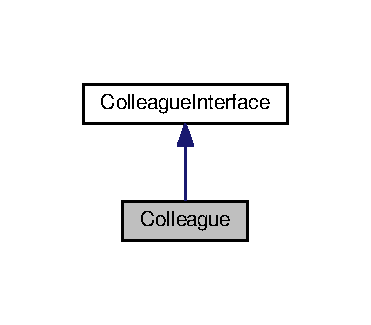
\includegraphics[width=178pt]{classColleague__inherit__graph}
\end{center}
\end{figure}


Collaboration diagram for Colleague\+:
\nopagebreak
\begin{figure}[H]
\begin{center}
\leavevmode
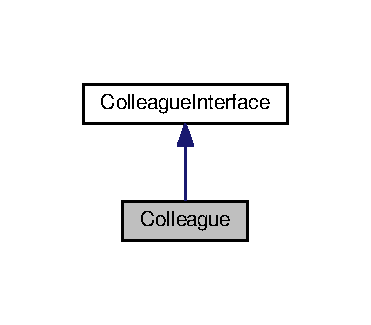
\includegraphics[width=178pt]{classColleague__coll__graph}
\end{center}
\end{figure}
\subsection*{Public Member Functions}
\begin{DoxyCompactItemize}
\item 
virtual void \hyperlink{classColleague_afb6563e15f8ea7f8931d5c51ad15cef6}{send\+Message} (const \hyperlink{classMediatorInterface}{Mediator\+Interface} \&, const std\+::string \&) const override
\end{DoxyCompactItemize}
\subsection*{Private Member Functions}
\begin{DoxyCompactItemize}
\item 
virtual void \hyperlink{classColleague_ac1834eb0fe9749f84294ef342b8370dc}{receive\+Message} (const \hyperlink{classColleagueInterface}{Colleague\+Interface} $\ast$, const std\+::string \&) const override
\end{DoxyCompactItemize}


\subsection{Member Function Documentation}
\index{Colleague@{Colleague}!receive\+Message@{receive\+Message}}
\index{receive\+Message@{receive\+Message}!Colleague@{Colleague}}
\subsubsection[{\texorpdfstring{receive\+Message(const Colleague\+Interface $\ast$, const std\+::string \&) const override}{receiveMessage(const ColleagueInterface *, const std::string &) const override}}]{\setlength{\rightskip}{0pt plus 5cm}void Colleague\+::receive\+Message (
\begin{DoxyParamCaption}
\item[{const {\bf Colleague\+Interface} $\ast$}]{sender, }
\item[{const std\+::string \&}]{message}
\end{DoxyParamCaption}
) const\hspace{0.3cm}{\ttfamily [override]}, {\ttfamily [private]}, {\ttfamily [virtual]}}\hypertarget{classColleague_ac1834eb0fe9749f84294ef342b8370dc}{}\label{classColleague_ac1834eb0fe9749f84294ef342b8370dc}


Implements \hyperlink{classColleagueInterface_ad54da6a768fff80244b2f81af95cdbc1}{Colleague\+Interface}.


\begin{DoxyCode}
41                                                                                                 \{
42     std::cout << \hyperlink{classColleagueInterface_acbc50603b8b5f9e94f36bb94a53fd651}{getName}() << \textcolor{stringliteral}{" received the message from "} << sender->
      \hyperlink{classColleagueInterface_acbc50603b8b5f9e94f36bb94a53fd651}{getName}() << \textcolor{stringliteral}{": "} << message << std::endl;           
43 \}
\end{DoxyCode}


Here is the call graph for this function\+:
\nopagebreak
\begin{figure}[H]
\begin{center}
\leavevmode
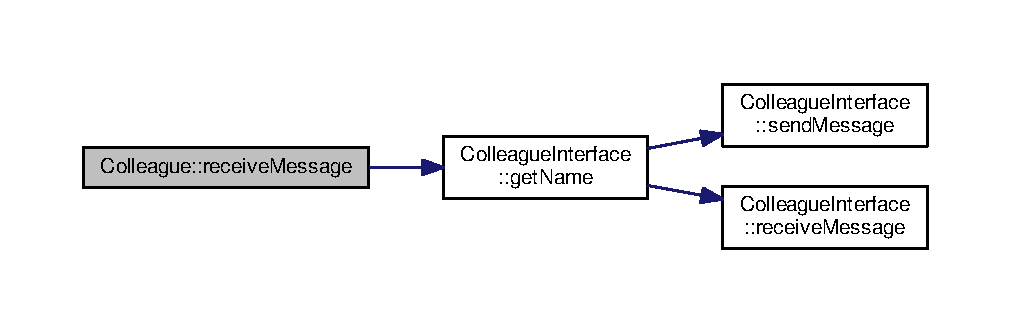
\includegraphics[width=350pt]{classColleague_ac1834eb0fe9749f84294ef342b8370dc_cgraph}
\end{center}
\end{figure}


\index{Colleague@{Colleague}!send\+Message@{send\+Message}}
\index{send\+Message@{send\+Message}!Colleague@{Colleague}}
\subsubsection[{\texorpdfstring{send\+Message(const Mediator\+Interface \&, const std\+::string \&) const override}{sendMessage(const MediatorInterface &, const std::string &) const override}}]{\setlength{\rightskip}{0pt plus 5cm}void Colleague\+::send\+Message (
\begin{DoxyParamCaption}
\item[{const {\bf Mediator\+Interface} \&}]{mediator, }
\item[{const std\+::string \&}]{message}
\end{DoxyParamCaption}
) const\hspace{0.3cm}{\ttfamily [override]}, {\ttfamily [virtual]}}\hypertarget{classColleague_afb6563e15f8ea7f8931d5c51ad15cef6}{}\label{classColleague_afb6563e15f8ea7f8931d5c51ad15cef6}


Implements \hyperlink{classColleagueInterface_a1b86fdff9280809073590a466280fd06}{Colleague\+Interface}.


\begin{DoxyCode}
37                                                                                               \{
38     mediator.\hyperlink{classMediatorInterface_a6445b79436acab5998b8a957648fadb1}{distributeMessage} (\textcolor{keyword}{this}, message);
39 \}
\end{DoxyCode}


Here is the call graph for this function\+:
\nopagebreak
\begin{figure}[H]
\begin{center}
\leavevmode
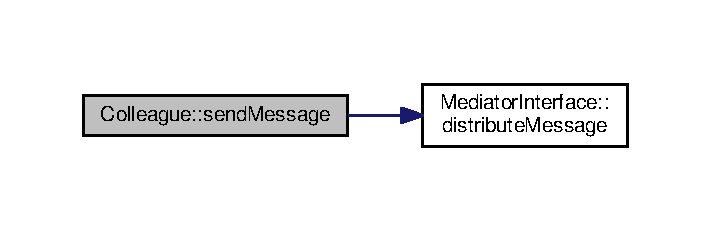
\includegraphics[width=341pt]{classColleague_afb6563e15f8ea7f8931d5c51ad15cef6_cgraph}
\end{center}
\end{figure}




The documentation for this class was generated from the following file\+:\begin{DoxyCompactItemize}
\item 
\hyperlink{Mediator_8cpp}{Mediator.\+cpp}\end{DoxyCompactItemize}

\hypertarget{classColleagueInterface}{}\section{Colleague\+Interface Class Reference}
\label{classColleagueInterface}\index{Colleague\+Interface@{Colleague\+Interface}}


Inheritance diagram for Colleague\+Interface\+:
\nopagebreak
\begin{figure}[H]
\begin{center}
\leavevmode
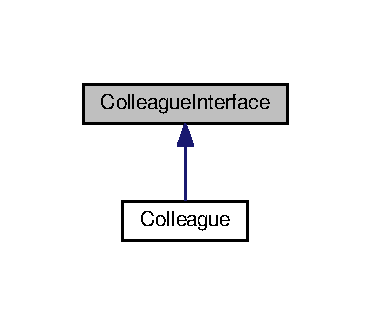
\includegraphics[width=178pt]{classColleagueInterface__inherit__graph}
\end{center}
\end{figure}
\subsection*{Public Member Functions}
\begin{DoxyCompactItemize}
\item 
\hyperlink{classColleagueInterface_a1615c154b4c9f05d7c35793acc170696}{Colleague\+Interface} (const std\+::string \&new\+Name)
\item 
std\+::string \hyperlink{classColleagueInterface_acbc50603b8b5f9e94f36bb94a53fd651}{get\+Name} () const 
\item 
virtual void \hyperlink{classColleagueInterface_a1b86fdff9280809073590a466280fd06}{send\+Message} (const \hyperlink{classMediatorInterface}{Mediator\+Interface} \&, const std\+::string \&) const =0
\item 
virtual void \hyperlink{classColleagueInterface_ad54da6a768fff80244b2f81af95cdbc1}{receive\+Message} (const \hyperlink{classColleagueInterface}{Colleague\+Interface} $\ast$, const std\+::string \&) const =0
\end{DoxyCompactItemize}
\subsection*{Private Attributes}
\begin{DoxyCompactItemize}
\item 
std\+::string \hyperlink{classColleagueInterface_aa5a767ee2b42271eadf388956525831b}{name}
\end{DoxyCompactItemize}


\subsection{Constructor \& Destructor Documentation}
\index{Colleague\+Interface@{Colleague\+Interface}!Colleague\+Interface@{Colleague\+Interface}}
\index{Colleague\+Interface@{Colleague\+Interface}!Colleague\+Interface@{Colleague\+Interface}}
\subsubsection[{\texorpdfstring{Colleague\+Interface(const std\+::string \&new\+Name)}{ColleagueInterface(const std::string &newName)}}]{\setlength{\rightskip}{0pt plus 5cm}Colleague\+Interface\+::\+Colleague\+Interface (
\begin{DoxyParamCaption}
\item[{const std\+::string \&}]{new\+Name}
\end{DoxyParamCaption}
)\hspace{0.3cm}{\ttfamily [inline]}}\hypertarget{classColleagueInterface_a1615c154b4c9f05d7c35793acc170696}{}\label{classColleagueInterface_a1615c154b4c9f05d7c35793acc170696}

\begin{DoxyCode}
10 : \hyperlink{classColleagueInterface_aa5a767ee2b42271eadf388956525831b}{name} (newName) \{\}
\end{DoxyCode}


\subsection{Member Function Documentation}
\index{Colleague\+Interface@{Colleague\+Interface}!get\+Name@{get\+Name}}
\index{get\+Name@{get\+Name}!Colleague\+Interface@{Colleague\+Interface}}
\subsubsection[{\texorpdfstring{get\+Name() const }{getName() const }}]{\setlength{\rightskip}{0pt plus 5cm}std\+::string Colleague\+Interface\+::get\+Name (
\begin{DoxyParamCaption}
{}
\end{DoxyParamCaption}
) const\hspace{0.3cm}{\ttfamily [inline]}}\hypertarget{classColleagueInterface_acbc50603b8b5f9e94f36bb94a53fd651}{}\label{classColleagueInterface_acbc50603b8b5f9e94f36bb94a53fd651}

\begin{DoxyCode}
11 \{\textcolor{keywordflow}{return} \hyperlink{classColleagueInterface_aa5a767ee2b42271eadf388956525831b}{name};\}
\end{DoxyCode}


Here is the call graph for this function\+:
\nopagebreak
\begin{figure}[H]
\begin{center}
\leavevmode
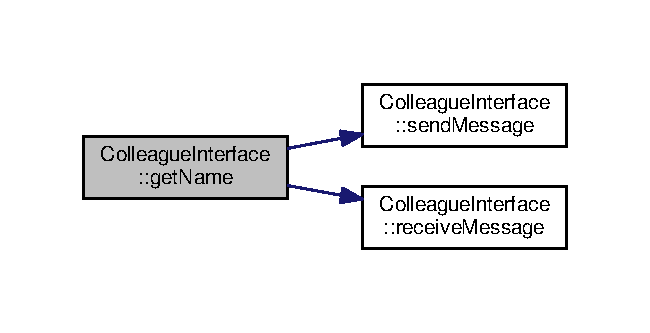
\includegraphics[width=312pt]{classColleagueInterface_acbc50603b8b5f9e94f36bb94a53fd651_cgraph}
\end{center}
\end{figure}


\index{Colleague\+Interface@{Colleague\+Interface}!receive\+Message@{receive\+Message}}
\index{receive\+Message@{receive\+Message}!Colleague\+Interface@{Colleague\+Interface}}
\subsubsection[{\texorpdfstring{receive\+Message(const Colleague\+Interface $\ast$, const std\+::string \&) const =0}{receiveMessage(const ColleagueInterface *, const std::string &) const =0}}]{\setlength{\rightskip}{0pt plus 5cm}virtual void Colleague\+Interface\+::receive\+Message (
\begin{DoxyParamCaption}
\item[{const {\bf Colleague\+Interface} $\ast$}]{, }
\item[{const std\+::string \&}]{}
\end{DoxyParamCaption}
) const\hspace{0.3cm}{\ttfamily [pure virtual]}}\hypertarget{classColleagueInterface_ad54da6a768fff80244b2f81af95cdbc1}{}\label{classColleagueInterface_ad54da6a768fff80244b2f81af95cdbc1}


Implemented in \hyperlink{classColleague_ac1834eb0fe9749f84294ef342b8370dc}{Colleague}.

\index{Colleague\+Interface@{Colleague\+Interface}!send\+Message@{send\+Message}}
\index{send\+Message@{send\+Message}!Colleague\+Interface@{Colleague\+Interface}}
\subsubsection[{\texorpdfstring{send\+Message(const Mediator\+Interface \&, const std\+::string \&) const =0}{sendMessage(const MediatorInterface &, const std::string &) const =0}}]{\setlength{\rightskip}{0pt plus 5cm}virtual void Colleague\+Interface\+::send\+Message (
\begin{DoxyParamCaption}
\item[{const {\bf Mediator\+Interface} \&}]{, }
\item[{const std\+::string \&}]{}
\end{DoxyParamCaption}
) const\hspace{0.3cm}{\ttfamily [pure virtual]}}\hypertarget{classColleagueInterface_a1b86fdff9280809073590a466280fd06}{}\label{classColleagueInterface_a1b86fdff9280809073590a466280fd06}


Implemented in \hyperlink{classColleague_afb6563e15f8ea7f8931d5c51ad15cef6}{Colleague}.



\subsection{Member Data Documentation}
\index{Colleague\+Interface@{Colleague\+Interface}!name@{name}}
\index{name@{name}!Colleague\+Interface@{Colleague\+Interface}}
\subsubsection[{\texorpdfstring{name}{name}}]{\setlength{\rightskip}{0pt plus 5cm}std\+::string Colleague\+Interface\+::name\hspace{0.3cm}{\ttfamily [private]}}\hypertarget{classColleagueInterface_aa5a767ee2b42271eadf388956525831b}{}\label{classColleagueInterface_aa5a767ee2b42271eadf388956525831b}


The documentation for this class was generated from the following file\+:\begin{DoxyCompactItemize}
\item 
\hyperlink{Mediator_8cpp}{Mediator.\+cpp}\end{DoxyCompactItemize}

\hypertarget{classMediator}{}\section{Mediator Class Reference}
\label{classMediator}\index{Mediator@{Mediator}}


Inheritance diagram for Mediator\+:
\nopagebreak
\begin{figure}[H]
\begin{center}
\leavevmode
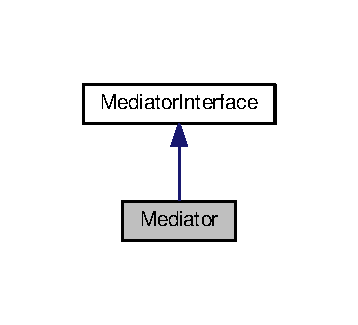
\includegraphics[width=172pt]{classMediator__inherit__graph}
\end{center}
\end{figure}


Collaboration diagram for Mediator\+:
\nopagebreak
\begin{figure}[H]
\begin{center}
\leavevmode
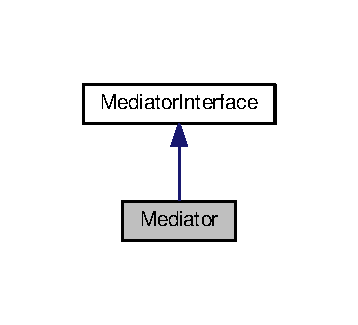
\includegraphics[width=172pt]{classMediator__coll__graph}
\end{center}
\end{figure}
\subsection*{Private Member Functions}
\begin{DoxyCompactItemize}
\item 
virtual void \hyperlink{classMediator_a6dafbc84aae81e04af696169924b04fc}{distribute\+Message} (const \hyperlink{classColleagueInterface}{Colleague\+Interface} $\ast$, const std\+::string \&) const override
\end{DoxyCompactItemize}
\subsection*{Additional Inherited Members}


\subsection{Member Function Documentation}
\index{Mediator@{Mediator}!distribute\+Message@{distribute\+Message}}
\index{distribute\+Message@{distribute\+Message}!Mediator@{Mediator}}
\subsubsection[{\texorpdfstring{distribute\+Message(const Colleague\+Interface $\ast$, const std\+::string \&) const override}{distributeMessage(const ColleagueInterface *, const std::string &) const override}}]{\setlength{\rightskip}{0pt plus 5cm}void Mediator\+::distribute\+Message (
\begin{DoxyParamCaption}
\item[{const {\bf Colleague\+Interface} $\ast$}]{sender, }
\item[{const std\+::string \&}]{message}
\end{DoxyParamCaption}
) const\hspace{0.3cm}{\ttfamily [override]}, {\ttfamily [private]}, {\ttfamily [virtual]}}\hypertarget{classMediator_a6dafbc84aae81e04af696169924b04fc}{}\label{classMediator_a6dafbc84aae81e04af696169924b04fc}


Implements \hyperlink{classMediatorInterface_a6445b79436acab5998b8a957648fadb1}{Mediator\+Interface}.


\begin{DoxyCode}
45                                                                                                   \{
46     \textcolor{keywordflow}{for} (\textcolor{keyword}{const} \hyperlink{classColleagueInterface}{ColleagueInterface}* x : \hyperlink{classMediatorInterface_ac7329ec51656cb23b2c41ada567570fc}{getColleagueList}())
47         \textcolor{keywordflow}{if} (x != sender)  \textcolor{comment}{// Do not send the message back to the sender}
48             x->receiveMessage (sender, message);
49 \}
\end{DoxyCode}


The documentation for this class was generated from the following file\+:\begin{DoxyCompactItemize}
\item 
\hyperlink{Mediator_8cpp}{Mediator.\+cpp}\end{DoxyCompactItemize}

\hypertarget{classMediatorInterface}{}\section{Mediator\+Interface Class Reference}
\label{classMediatorInterface}\index{Mediator\+Interface@{Mediator\+Interface}}


Inheritance diagram for Mediator\+Interface\+:
\nopagebreak
\begin{figure}[H]
\begin{center}
\leavevmode
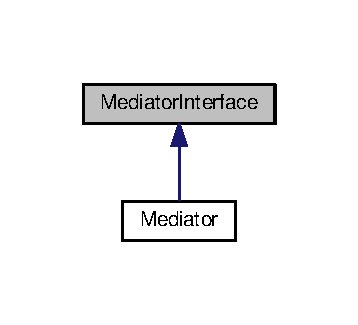
\includegraphics[width=172pt]{classMediatorInterface__inherit__graph}
\end{center}
\end{figure}
\subsection*{Public Member Functions}
\begin{DoxyCompactItemize}
\item 
const std\+::list$<$ \hyperlink{classColleagueInterface}{Colleague\+Interface} $\ast$ $>$ \& \hyperlink{classMediatorInterface_ac7329ec51656cb23b2c41ada567570fc}{get\+Colleague\+List} () const 
\item 
virtual void \hyperlink{classMediatorInterface_a6445b79436acab5998b8a957648fadb1}{distribute\+Message} (const \hyperlink{classColleagueInterface}{Colleague\+Interface} $\ast$, const std\+::string \&) const =0
\item 
virtual void \hyperlink{classMediatorInterface_acf4de17fcada54c6701c2afb11c754bd}{register\+Colleague} (\hyperlink{classColleagueInterface}{Colleague\+Interface} $\ast$colleague)
\end{DoxyCompactItemize}
\subsection*{Private Attributes}
\begin{DoxyCompactItemize}
\item 
std\+::list$<$ \hyperlink{classColleagueInterface}{Colleague\+Interface} $\ast$ $>$ \hyperlink{classMediatorInterface_a6bb9dcea81ba62644bcaec1bf590cb42}{colleague\+List}
\end{DoxyCompactItemize}


\subsection{Member Function Documentation}
\index{Mediator\+Interface@{Mediator\+Interface}!distribute\+Message@{distribute\+Message}}
\index{distribute\+Message@{distribute\+Message}!Mediator\+Interface@{Mediator\+Interface}}
\subsubsection[{\texorpdfstring{distribute\+Message(const Colleague\+Interface $\ast$, const std\+::string \&) const =0}{distributeMessage(const ColleagueInterface *, const std::string &) const =0}}]{\setlength{\rightskip}{0pt plus 5cm}virtual void Mediator\+Interface\+::distribute\+Message (
\begin{DoxyParamCaption}
\item[{const {\bf Colleague\+Interface} $\ast$}]{, }
\item[{const std\+::string \&}]{}
\end{DoxyParamCaption}
) const\hspace{0.3cm}{\ttfamily [pure virtual]}}\hypertarget{classMediatorInterface_a6445b79436acab5998b8a957648fadb1}{}\label{classMediatorInterface_a6445b79436acab5998b8a957648fadb1}


Implemented in \hyperlink{classMediator_a6dafbc84aae81e04af696169924b04fc}{Mediator}.

\index{Mediator\+Interface@{Mediator\+Interface}!get\+Colleague\+List@{get\+Colleague\+List}}
\index{get\+Colleague\+List@{get\+Colleague\+List}!Mediator\+Interface@{Mediator\+Interface}}
\subsubsection[{\texorpdfstring{get\+Colleague\+List() const }{getColleagueList() const }}]{\setlength{\rightskip}{0pt plus 5cm}const std\+::list$<${\bf Colleague\+Interface}$\ast$$>$\& Mediator\+Interface\+::get\+Colleague\+List (
\begin{DoxyParamCaption}
{}
\end{DoxyParamCaption}
) const\hspace{0.3cm}{\ttfamily [inline]}}\hypertarget{classMediatorInterface_ac7329ec51656cb23b2c41ada567570fc}{}\label{classMediatorInterface_ac7329ec51656cb23b2c41ada567570fc}

\begin{DoxyCode}
28 \{\textcolor{keywordflow}{return} \hyperlink{classMediatorInterface_a6bb9dcea81ba62644bcaec1bf590cb42}{colleagueList};\}
\end{DoxyCode}
\index{Mediator\+Interface@{Mediator\+Interface}!register\+Colleague@{register\+Colleague}}
\index{register\+Colleague@{register\+Colleague}!Mediator\+Interface@{Mediator\+Interface}}
\subsubsection[{\texorpdfstring{register\+Colleague(\+Colleague\+Interface $\ast$colleague)}{registerColleague(ColleagueInterface *colleague)}}]{\setlength{\rightskip}{0pt plus 5cm}virtual void Mediator\+Interface\+::register\+Colleague (
\begin{DoxyParamCaption}
\item[{{\bf Colleague\+Interface} $\ast$}]{colleague}
\end{DoxyParamCaption}
)\hspace{0.3cm}{\ttfamily [inline]}, {\ttfamily [virtual]}}\hypertarget{classMediatorInterface_acf4de17fcada54c6701c2afb11c754bd}{}\label{classMediatorInterface_acf4de17fcada54c6701c2afb11c754bd}

\begin{DoxyCode}
30 \{\hyperlink{classMediatorInterface_a6bb9dcea81ba62644bcaec1bf590cb42}{colleagueList}.emplace\_back (colleague);\}
\end{DoxyCode}


\subsection{Member Data Documentation}
\index{Mediator\+Interface@{Mediator\+Interface}!colleague\+List@{colleague\+List}}
\index{colleague\+List@{colleague\+List}!Mediator\+Interface@{Mediator\+Interface}}
\subsubsection[{\texorpdfstring{colleague\+List}{colleagueList}}]{\setlength{\rightskip}{0pt plus 5cm}std\+::list$<${\bf Colleague\+Interface}$\ast$$>$ Mediator\+Interface\+::colleague\+List\hspace{0.3cm}{\ttfamily [private]}}\hypertarget{classMediatorInterface_a6bb9dcea81ba62644bcaec1bf590cb42}{}\label{classMediatorInterface_a6bb9dcea81ba62644bcaec1bf590cb42}


The documentation for this class was generated from the following file\+:\begin{DoxyCompactItemize}
\item 
\hyperlink{Mediator_8cpp}{Mediator.\+cpp}\end{DoxyCompactItemize}

\chapter{File Documentation}
\hypertarget{Mediator_8cpp}{}\section{Mediator.\+cpp File Reference}
\label{Mediator_8cpp}\index{Mediator.\+cpp@{Mediator.\+cpp}}
{\ttfamily \#include $<$iostream$>$}\\*
{\ttfamily \#include $<$string$>$}\\*
{\ttfamily \#include $<$list$>$}\\*
Include dependency graph for Mediator.\+cpp\+:
\nopagebreak
\begin{figure}[H]
\begin{center}
\leavevmode
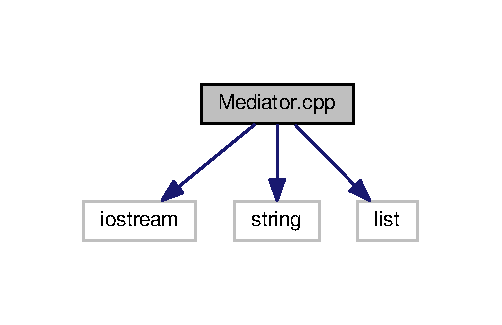
\includegraphics[width=241pt]{Mediator_8cpp__incl}
\end{center}
\end{figure}
\subsection*{Classes}
\begin{DoxyCompactItemize}
\item 
class \hyperlink{classColleagueInterface}{Colleague\+Interface}
\item 
class \hyperlink{classColleague}{Colleague}
\item 
class \hyperlink{classMediatorInterface}{Mediator\+Interface}
\item 
class \hyperlink{classMediator}{Mediator}
\end{DoxyCompactItemize}
\subsection*{Functions}
\begin{DoxyCompactItemize}
\item 
int \hyperlink{Mediator_8cpp_ae66f6b31b5ad750f1fe042a706a4e3d4}{main} ()
\end{DoxyCompactItemize}


\subsection{Function Documentation}
\index{Mediator.\+cpp@{Mediator.\+cpp}!main@{main}}
\index{main@{main}!Mediator.\+cpp@{Mediator.\+cpp}}
\subsubsection[{\texorpdfstring{main()}{main()}}]{\setlength{\rightskip}{0pt plus 5cm}int main (
\begin{DoxyParamCaption}
{}
\end{DoxyParamCaption}
)}\hypertarget{Mediator_8cpp_ae66f6b31b5ad750f1fe042a706a4e3d4}{}\label{Mediator_8cpp_ae66f6b31b5ad750f1fe042a706a4e3d4}

\begin{DoxyCode}
51            \{
52     \hyperlink{classColleague}{Colleague} *bob = \textcolor{keyword}{new} \hyperlink{classColleague}{Colleague} (\textcolor{stringliteral}{"Bob"}),  *sam = \textcolor{keyword}{new} 
      \hyperlink{classColleague}{Colleague} (\textcolor{stringliteral}{"Sam"}),  *frank = \textcolor{keyword}{new} \hyperlink{classColleague}{Colleague} (\textcolor{stringliteral}{"Frank"}),  *tom = \textcolor{keyword}{new} 
      \hyperlink{classColleague}{Colleague} (\textcolor{stringliteral}{"Tom"});
53     \hyperlink{classColleague}{Colleague}* staff[] = \{bob, sam, frank, tom\};
54     \hyperlink{classMediator}{Mediator} mediatorStaff, mediatorSamsBuddies;
55     \textcolor{keywordflow}{for} (\hyperlink{classColleague}{Colleague}* x : staff)
56         mediatorStaff.\hyperlink{classMediatorInterface_acf4de17fcada54c6701c2afb11c754bd}{registerColleague}(x);
57     bob->\hyperlink{classColleague_afb6563e15f8ea7f8931d5c51ad15cef6}{sendMessage} (mediatorStaff, \textcolor{stringliteral}{"I'm quitting this job!"});
58     mediatorSamsBuddies.\hyperlink{classMediatorInterface_acf4de17fcada54c6701c2afb11c754bd}{registerColleague} (frank);  mediatorSamsBuddies.
      \hyperlink{classMediatorInterface_acf4de17fcada54c6701c2afb11c754bd}{registerColleague} (tom);  \textcolor{comment}{// Sam's buddies only}
59     sam->sendMessage (mediatorSamsBuddies, \textcolor{stringliteral}{"Hooray!  He's gone!  Let's go for a drink, guys!"}); 
60     \textcolor{keywordflow}{return} 0;
61 \}\end{DoxyCode}


Here is the call graph for this function\+:
\nopagebreak
\begin{figure}[H]
\begin{center}
\leavevmode
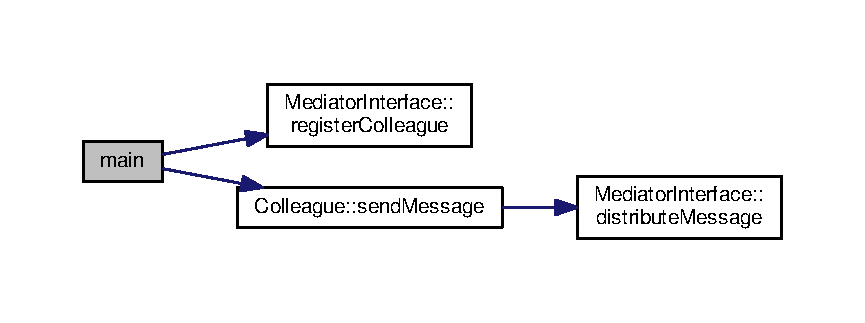
\includegraphics[width=350pt]{Mediator_8cpp_ae66f6b31b5ad750f1fe042a706a4e3d4_cgraph}
\end{center}
\end{figure}



%--- End generated contents ---

% Index
\backmatter
\newpage
\phantomsection
\clearemptydoublepage
\addcontentsline{toc}{chapter}{Index}
\printindex

\end{document}
